\chapter{Implementación}
Como se ha comentado en capítulos anteriores la implementación del software se ha desarrollado en el lenguaje de programación M, propio de Matlab y con el entorno de creación de interfaces de usuario GUIDE.

\bigskip

\section{Implementación de la interfaz gráfica}

Finalmente la GUI creada sigue los patrones estéticos diseñados en el capítulo anterior con pequeñas modificaciones para una mayor claridad y la inclusión de dos nuevos campos en la sección de visualización.

\begin{figure}[H]
\centering
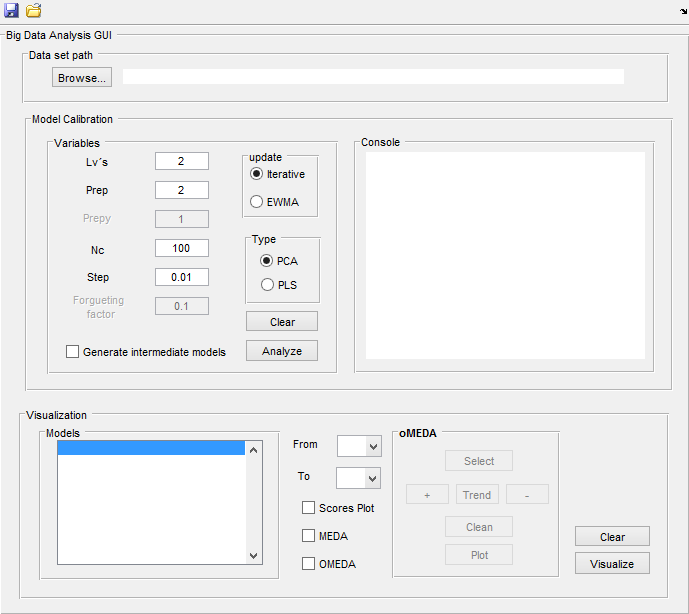
\includegraphics[width=0.7\textwidth]{imagenes/figuras/9_1.png}
\caption{GUI final.}
\end{figure}

\bigskip

Como se puede observar en la figura 9.1 los cambios introducidos con respecto al diseño son mínimos, simplemente se han añadido unas etiquetas en cada uno de los paneles separadores identificando qué se hace dentro de cada uno de ellos, y unos botones de guardado del entorno y de carga de entornos guardados con anterioridad, además de dos menús desplegables para la selección de las componentes principales a visualizar.

\begin{figure}
\centering
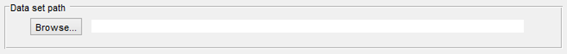
\includegraphics[width=0.9\textwidth]{imagenes/figuras/9_2.png}
\caption{Ruta a los datos.}
\end{figure}

\bigskip

La figura 9.2 muestra la zona de la GUI donde se selecciona el conjunto de datos a analizar de un fichero “.mat”.

\begin{figure}
\centering
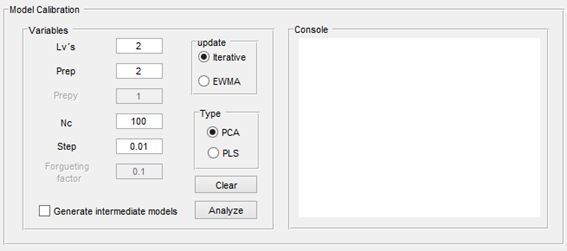
\includegraphics[width=0.9\textwidth]{imagenes/figuras/9_3.png}
\caption{Calibración del modelo.}
\end{figure}

\bigskip

En la figura 9.3 se puede ver la zona central de la interfaz, que aúna el módulo funcional de calibración del modelo con el de análisis, aunque como se verá más adelante en el código están separadas en dos funciones independientes.

\bigskip

Cada uno de los campos de la subsección “Variables” se explicaron con anterioridad en el capítulo 3.
\bigskip

En la subsección “Console” irán apareciendo todas las salidas que mostraría la aplicación al ejecutarse por terminal. 

\begin{figure}
\centering
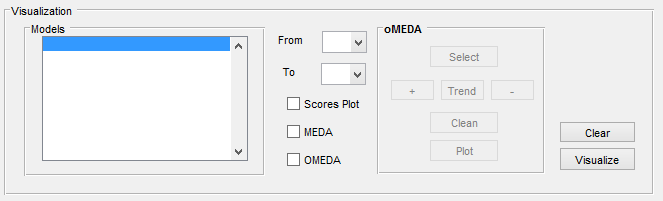
\includegraphics[width=0.9\textwidth]{imagenes/figuras/9_4.png}
\caption{Visualización.}
\end{figure}

\bigskip

En la figura 9.4 se puede ver la subsección de “Visualization”, en la que se mostraran los modelos ya calibrados y estructurados mediantes los análisis correspondientes para poder visualizarlos en Score Plots, MEDA y oMEDA. El apartado oMEDA permite seleccionar los puntos a mostrar en el gráfico. Este apartado fué desarrollado por Elena Jimenez Mañas \cite{PHPDAT} y en el presente trabajo se ha adaptado para el manejo de Big Data. Los campos From y To son para seleccionar desde qué componente a qué otro se desea visualizar.


\section{Código desarrollado}

En esta sección se va a explicar el código desarrollado para los módulos comentados en la fase de diseño. Como se dijo anteriormente la fase de calibración del modelo y la de análisis se han fusionado en lo que a interfaz gráfica se refiere, pero el código de ambas funciones está separado.

\bigskip

La función \textbf{modelCalibration} se encarga de comprobar que todos los campos introducidos en la sección del mismo nombre de la GUI sean correctos y almacena los necesarios en variables globales para su uso continuo. Si alguno  de los campos no tiene valor lanza un mensaje de error pidiendo que se rellene para poder seguir adelante.
\bigskip

Tras confirmar que todos los campos han sido rellenados pasa a incializar el primero modelo con los datos proporcionados por el usuario y por último rellena las listas From y To del apartado Visualization con los componentes principales generados en función del campo Lvs.
\bigskip


la función \textbf{Analize}, comienza tomando las variables globales necesarias para llevar a cabo las tareas que se tienen que desarrollar en la misma, rellenas ya con los valores necesarios en modelCalibration.

\bigskip

A continuación se carga el fichero de datos introducido en la sección Data set Path, y según los campos seleccionados de la zona Model calibration de la GUI se va generando el primero modelo, a partir del cuál se generarán los demás si se ha seleccionado la opción Generate intermediate models, o se generará sólo ese si no se ha seleccionado dicha opción.

\bigskip

Si se ha seleccionado la opción Generate intermediate models se pasa a crear una lista con los nombres que se le van a dar a cada uno de los modelos, que cuando se termine el proceso aparecerá en el listboxModels del apartado de Visualization para poder seleccionar el que se desee para su visualización.

\bigskip

Una vez hecho esto se actualiza el primer modelo con la funcion update\_iterative2 o update\_ewma2 en función de la opción seleccionada en Model Calibration y a continuación se entra en un bucle que irá generando tantos modelos como ficheros de datos se tengan. Cada modelo se genera en función del anterior por ello el bucle comienza en 2 y termina en el tamaño de la lista que contenga el fichero índice.

\bigskip

En caso de que se quiera generar un sólo modelo el código es mas simple, sólo se toman los campos necesarios de las variables globales y se actualiza el modelo en función de las opciones seleccionadas.
\bigskip

La función \textbf{Visualize} se encarga de tomar los modelos generados y visualizar el que se ha seleccionado mediante las gráficas elegidas.

\bigskip

En primer lugar esta función toma la lista de modelos globales, a continuación comprueba que los campos From y To no tengan el mismo valor, y en caso de ser así lanza un mensaje de error y cancela la visualización.Tras esto compara los valores de From y To para almacenar el menor y el mayor de los componentes principales de la selección para así poder llevar a cabo la visualización correctamente cuando son listas de componentes múltiples.Después comprueba que exista mas de un modelo para poder seleccionar de la lista, y en caso de no ser así marca como seleccionado el único que hay.

\bigskip

Una vez hecho todo lo anterior se pasa a generar las gráficas en función del los campos seleccionados en la sección visualization. Si se ha elegido crear un scoreplot se almacenaran las salidas que produzca este (matrices de puntos) en la variable T para su posterior utilización en oMEDA, se marcará cada gráfica con el tag ScorePlot para poder identificarlo y se llamará a la función \textbf{preparaOmeda}. Por último si se ha marcado MEDA también se generará.
\bigskip

La función \textbf{preparaOmeda} se encarga de inicializar una serie de variables que se utilizarán para poder localizar los puntos que se seleccionarán del ScorePlot para generar el oMEDA. Esta función forma parte del código desarrollado por Elena Jiménez Mañas y no se ha modificado nada en el presente trabajo.

\bigskip

Las funciones asociadas a los eventos de pulsación de todos los botones de la subsección oMEDA fueron desarrolladas y explicadas en el PFC "Herramientas para la detección de ataques en tráfico de red" de Elena Jiménez Mañas.